%
% CHAPTER 5.- The MDL Principle
%

\chapterimage{TuringMachine.pdf} % Chapter heading image

\chapter{Learning}
\label{ch:Learning}

\begin{quote}
\begin{flushright}
\emph{Some mathematical statements are true for no reason,\\
they're true by accident.}\\
Gregory Chaitin
\end{flushright}
\end{quote}
\bigskip

{\color{red} Warning: This section still requires a significant amount of work!}

Machine learning refers to a large collection of algorithms designed to automatically build mathematical models based on sample data sets, usually with the aim of making predictions, classifying objects, or simply to better understand the structure of the data. In the past decade, machine learning algorithms have been highly successful in areas like self-driving cars, practical speech recognition, effective web search, and purchase recommendations.

In this chapter we are going to see how the problem of learning from data is formally formulated in the area of machine learning. In this sense, the chapter is a continuation of the introduction to discrete probability included in Section \ref{sec:discrete_probability}. Also, we are going to study in detail two particular approaches to machine learning that are highly related to our theory of nescience: the Minimum Description Length principle and the Minimum Message Length principle.

Most of the learning algorithms used today in practice are known since forty years ago. The high success of current machine learning applications is largely due to the availability of huge, high-quality, training datasets, and to the advance of computing power, and in particular, thanks to the powerful graphical processing units (GPU) used in video-games. In Chapter \ref{chap:Machine-Learning} we will introduce a collection of new machine learning algorithms based on the theory of nescience, and we will compare them with the current, state of the art, algorithms.

%
% Statistical Inference
%

\section{Statistical Inference}

\emph{Statistical inference}\index{Statistical inference} has traditionally been presented as the way to make sense of reality through data. It applies probabilistic models to relate finite observations to broader populations, aiming to offer predictions and structured conclusions. However, statistical inference is not a direct reflection of reality but rather a tool that depends heavily on assumptions and idealized models. These models simplify complex phenomena, and the validity of their conclusions relies on how well these assumptions align with the underlying data-generating processes.

The random sampling model serves as a stepwise framework in statistical inference, guiding how we connect finite samples to broader populations:

Step 1.- Defining the Population and Collecting Data: The first step is to define the population of interest and determine how data will be collected. This involves specifying the sampling process and ensuring that each data point is drawn independently and identically distributed (iid) from the same population, with every unit having a nonzero probability of selection. Once the sampling process is defined, data is collected as a sample from the population, and each observation is treated as a realization of a random variable following the specified distribution.

Step 2.- Constructing and Checking the Random Sampling Model: Based on the assumptions about how the data was generated, the random sampling model is mathematically expressed. For example, , where  is the unknown population distribution with parameter . This step formalizes the relationship between the data and the population. Real-world data rarely fits these idealized assumptions perfectly, so it is essential to check for deviations such as selection biases or lack of independence and address them appropriately.

Step 3.- Applying the Likelihood Function and Estimating Parameters: The likelihood function plays a central role in parameter estimation by quantifying how plausible different parameter values are given the observed data . Methods such as maximum likelihood estimation (MLE) or Bayesian inference refine these estimates, translating raw data into structured knowledge about the population. For example, the sample mean  is often used as an estimate of the population mean .

Step 4.- Quantifying Uncertainty and Generalizing to the Population: Recognizing that the sample is just one realization of a random process, uncertainty must be quantified to understand how sample statistics behave across repeated samples. Sampling distributions, confidence intervals, and hypothesis tests help describe this variability. The Central Limit Theorem ensures that for large samples, the sample mean  approximates a normal distribution, making inference more reliable. Finally, results are generalized from the sample to the population using frequentist methods such as confidence intervals and p-values or Bayesian methods that update beliefs about  by incorporating prior knowledge.

The random sampling model provides a structured, step-by-step approach for making inferences from data. However, each step depends on assumptions that rarely hold perfectly in practice. As such, conclusions drawn from statistical inference should be viewed as tentative and context-dependent, subject to revision when new data or insights become available.

\begin{definition}
A \emph{statistical model}\index{Statistical model} is a random variable, together with a specification of its probability distribution, and the identification of the parameters, denoted by $\theta$, of that distribution.
\end{definition}

A statistic is a function of the observable data. A statistic is used to summarize or describe some aspect of the sample. For example, the sample mean and the sample variance are statistics because they summarize data drawn from a sample.

\begin{definition}
Let $\mathbf{X}=\left(X_{1},\ldots,X_{n}\right)$ be a random sample. A \emph{statistic}\index{Statistic} is a random variable $T = r \left( X_1, \ldots, X_n \right)$, where $r()$ is an arbitrary real-valued function of $n$ variables.
\end{definition}

A \emph{parametric random variable}\index{Parametric random variable} is a random variable $X$ that belongs to a family of functions parameterized by $\theta$. The parameter $\theta$ can either be a single scalar or a vector of values, and it is treated itself as a random variable that follows a probability distribution. The set $\Theta = \{ \theta_1, \theta_2, \ldots \}$, consisting of all possible values of $\theta$, is called the \emph{parameter space}\index{Parameter space}, and its elements are referred to as \emph{parameters}\index{Parameter of a probability distribution}. When the parameter $\theta$ is unknown, the distribution of the random variable $X$ is said to be conditional on $\theta$, denoted by $f\left(X \mid \theta \right)$.

As was the case in Chapter \ref{chap:Probability Theory}, in this section, we are only considering parametric discrete random variables defined over discrete probability spaces.

\begin{example}
We have seen in Definition \ref{def:binomial_distribution} that a binomial distribution with parameters $n$ and $p$ is a model for a family of experiments in which we are interested in knowing the number of successes in a sequence of $n$ independent binary trials, where the probability of success is $p$. If $X$ is a random variable following a binomial distribution, the probability of getting exactly $k$ successes is given by:
\[
Pr(X=k) = {\binom {n}{k}}p^{k}(1-p)^{n-k}
\]
In statistical inference, we are usually interested in the inverse problem. That is, we have the actual result of an experiment composed of $n$ trials, in which we know how many successes $k$ we have obtained, and we would like to estimate the parameter $p$, that is, the probability of success.
\end{example}

We assume that the true value of the unknown parameter $\theta$ can be inferred, typically by analyzing a collection of data samples. The observable data $\mathbf{X}=\left(X_{1},\ldots,X_{n}\right)$ is modeled as a random sample from the distribution $f\left(X \mid \theta \right)$ conditional on $\theta$.

An estimator of a parameter $\theta$ is a function of the random sample $\mathbf{X}$ that we hope provides a value close to the unknown parameter $\theta$.

\begin{definition}
Let $\mathbf{X}=\left(X_{1},\ldots,X_{n}\right)$ be a random sample from a discrete random variable $X$ with parameter $\theta$. An \emph{estimator}\index{Estimator} of the parameter $\theta$ is a real-valued function $\delta\left( X_1, \ldots, X_n \right)$. If $X_1 = x_1, \ldots, X_n = x_n$ are observed, then $\delta\left( x_1, \ldots, x_n \right)$ is called the \emph{estimate}\index{Estimate} of $\theta$.
\end{definition}

The estimator itself is a random variable, and its probability distribution can be derived from the joint distribution of $X_1, \ldots, X_n$. Every estimator is a statistic, but not every statistic is an estimator. The estimate is a real number.

Estimators help us estimate the quantities of interest in statistical inference and quantitatively assess the quality of the results. A good estimator is one where it is highly likely that the error $\delta(\mathbf{X}) - \theta$ will be close to zero.

In practice, we begin our analysis by deriving a distribution for the parameter $\theta$ based on theoretical assumptions and our current knowledge of the experiment.

When selecting an estimator, it is important to measure how "good" an estimate is. One common approach is to quantify the loss or cost associated with choosing an estimate that deviates from the true parameter value. This is done using a loss function, which assigns a numerical penalty to the difference between the estimate and the actual parameter.

\begin{definition}
A loss function is a real-valued function of two variables, $L\left(\theta,a\right)$, where $\theta \in \Theta$ and $a$ is a real number.
\end{definition}

The loss function represents the cost incurred when the true parameter value is $\theta$ and the estimate is $a$. In other words, $L\left(\theta,a\right)$ quantifies the loss when there is a discrepancy between the estimate and the true value.

Let $\xi\left(\theta\right)$ denote the prior probability mass function (p.m.f.) of $\theta$ on the set $\Theta$. Given a particular estimate $a$, the expected loss for discrete random variables is computed as:
\[
E\left[L\left(\theta,a\right)\right]=\sum_{\theta \in \Theta} L\left(\theta,a\right)\xi\left(\theta\right)
\]
The expected loss is the weighted average of the losses, where the weights are the probabilities $\xi(\theta)$ assigned to each possible value of $\theta$. The goal is to choose an estimate $a$ that minimizes this expected loss.

{\color{red}
The loss function $L\left(\theta,a\right)=\left(\theta-a\right)^{2}$ is called squared error loss. Let $\theta$ be a real-valued parameter. Suppose that the squared error loss function is used and that the posterior mean of $\theta$, $E\left(\theta\mid\mathbf{X}\right)$, is finite. Then, a Bayes estimator of $\theta$ is $\delta^{\ast}\left(\mathbf{X}\right)=E\left(\theta\mid\mathbf{X}\right)$.

The loss function $L\left(\theta,a\right)=\left|\theta-a\right|$ is called absolute error loss. When the absolute error loss function is used, a Bayes estimator of a real-valued parameter $\delta^{\ast}\left(\mathbf{X}\right)$ equal to a median of the posterior distribution of $\theta$.
}

% Maximum likelihood estimator

\subsection{Maximum Likelihood Estimator}

The Maximum Likelihood Estimator (abreviated MLE) is a method of estimating the parameters of a probability model. It is one of the most commonly used techniques in statistics for fitting model parameters to observed data. The core idea behind MLE is to find the parameter values that maximize a likelihood function, which represents the probability of observing the given data under the model. MLE is widely used due to its desirable properties for large samples, but its effectiveness relies on correct model specification and may struggle with small sample sizes or computational difficulties.

The likelihood represents the probability (or likelihood) of observing the data as a function of the parameters of the model.

\begin{definition}
Let \( X_1, X_2, \dots, X_n \) be $n$ independent and identically distributed discrete random variables, and let \( P(X_i = x_i \mid \theta) \) be the probability mass function of \( X_i \), where \( \theta \in \Theta \) is an unknown parameter, and \( \Theta \) is the parameter space. The \emph{likelihood function}\index{Likelihood function} is then defined as:
\[
L(\theta \mid X_1, X_2, \dots, X_n) = \prod_{i=1}^{n} P(X_i = x_i \mid \theta)
\]
where \( x_1, x_2, \dots, x_n \) are the observed data points.
\end{definition}

The likelihood function is a product of probabilities. Taking the logarithm of the likelihoodm, what it is called the \emph{log-likelihood function}\index{Log-likelihood function}, simplifies this product into a sum:
\[
\ell(\theta \mid X_1, X_2, \dots, X_n) = \log L(\theta \mid X_1, X_2, \dots, X_n) = \sum_{i=1}^{n} \log f(X_i \mid \theta)
\]
Sums are generally much easier to work with than products, particularly when performing differentiation for optimization purposes. This transformation makes it more straightforward to compute derivatives and apply optimization algorithms.

Maximum likelihood estimation is a method that determines values for the parameters of a model. The parameter values are found such that they maximise the likelihood that the process described by the model produced the data that were actually observed.

\begin{definition}
The \emph{Maximum Likelihood Estimator}\index{Maximum Likelihood Estimator}, abreviated as MLE, for discrete random variables is defined as the parameter value that maximizes the likelihood function, i.e.,
\[
\hat{\theta}_n = \arg \max_{\theta \in \Theta} L(\theta \mid X_1, X_2, \dots, X_n)
\]
\end{definition}

Equivalently, the MLE can also be found by maximizing the log-likelihood function:
\[
\hat{\theta}_n = \arg \max_{\theta \in \Theta} \ell(\theta \mid X_1, X_2, \dots, X_n)
\]

\begin{example}
Consider \( X_1, X_2, \dots, X_n \) i.i.d. random variables from a Bernoulli distribution with parameter \( p \). The probability mass function is:
\[
P(X_i = x_i \mid p) = p^{x_i}(1 - p)^{1 - x_i}
\]
where \( X_i \in \{0, 1\} \). The likelihood function for this sample is:
\[
L(p \mid X_1, X_2, \dots, X_n) = \prod_{i=1}^{n} p^{X_i}(1 - p)^{1 - X_i}
\]
Which can be rewritten as:
\[
L(p) = p^S (1 - p)^{n - S}
\]
where \( S = \sum_{i=1}^{n} X_i \) is the total number of successes (number of times \( X_i = 1 \)).  The function \( f(p) = p^a (1 - p)^b \) attains its maximum at \( p = \dfrac{a}{a + b} \). In our case, \( a = S \) and \( b = n - S \), so the likelihood function \( L(p) \) reaches its maximum at:
\[
\hat{p} = \dfrac{S}{S + (n - S)} = \dfrac{S}{n}
\]
Therefore, the maximum likelihood estimator for \( p \) is:
\[
\hat{p} = \dfrac{1}{n} \sum_{i=1}^{n} X_i
\]
which is simply the sample mean of the Bernoulli trials (the proportion of successes).
\end{example}

The maximun likelihood estimator is consitant.

\begin{proposition}
Let \( \hat{\theta}_n \) be the MLE for \( \theta \) when the random variables are discrete. Under regularity conditions (such as identifiability of the model and the existence of a unique maximizer of the likelihood function), the MLE is consistent, i.e.,
\[
\hat{\theta}_n \xrightarrow{\text{P}} \theta_0 \quad \text{as} \quad n \to \infty
\]
where \( \theta_0 \) is the true value of the parameter.
\end{proposition}
\begin{proof}
{\color{red} TODO: Finish}
1. Show that the expected log-likelihood is maximized at the true parameter \( \theta_0 \).
2. Prove that the empirical likelihood function converges uniformly to the expected log-likelihood as the sample size increases.
3. Establish that \( \hat{\theta}_n \) converges to \( \theta_0 \) as \( n \to \infty \).
\end{proof}

The MLE has several notable disadvantages. Firstly, it is highly dependent on sample size; for small samples, MLE may exhibit bias or high variance, as its desirable asymptotic properties, such as consistency, are guaranteed only for large datasets. Additionally, MLE requires correct model specification. It is sensitive to assumptions about the underlying model, and if the model is misspecified, the resulting estimates can be misleading. From a computational perspective, maximizing the likelihood function can pose numerical challenges, often necessitating complex optimization techniques that are computationally demanding and may result in convergence to local rather than global maxima. Furthermore, MLE is sensitive to outliers; since it seeks to maximize the likelihood based on observed data, extreme values can disproportionately affect the estimates, leading to distortions.

\begin{example}
Consider a situation where we are dealing with a uniform distribution \( U(0, \theta) \), where \( \theta \) is the unknown upper bound of the distribution. We have a sample \( X_1, X_2, \dots, X_n \) of i.i.d. observations from this distribution, and we wish to estimate the parameter \( \theta \) using the maximum likelihood estimator. The log-likelihood function is:
\[
\ell(\theta \mid X_1, X_2, \dots, X_n) = -n \log \theta, \quad \text{subject to} \quad \theta \geq \max(X_1, X_2, \dots, X_n)
\]
To maximize the log-likelihood, observe that \( \ell(\theta) \) is a decreasing function of \( \theta \). Therefore, the maximum likelihood occurs when \( \theta \) is minimized, subject to the constraint \( \theta \geq \max(X_1, X_2, \dots, X_n) \). Hence, the MLE for \( \theta \) is:
\[
\hat{\theta} = \max(X_1, X_2, \dots, X_n)
\]
The MLE \( \hat{\theta} \) tends to underestimate the true value of \( \theta \) when the sample size is small. This is because the maximum observation in a sample is unlikely to exactly reach the true upper bound, leading to a systematic bias. For example, if \( \theta = 10 \) and we take a sample of size 5, the expected value of \( \hat{\theta} \) is \( \frac{5}{6} \cdot 10 = 8.33 \), meaning we systematically underestimate the true parameter.

Since the MLE depends only on the maximum observed value, the estimate \( \hat{\theta} \) is highly sensitive to outliers. If an unusually large value appears in the sample, it can drastically inflate the estimate of \( \theta \), even if the rest of the data suggests a much smaller upper bound. This makes the MLE fragile in the presence of anomalous observations.

Another issue with the MLE in this case is that it ignores most of the data. The MLE is solely determined by the largest value in the sample, meaning the other \( n-1 \) data points do not contribute to the estimate. This seems inefficient because the estimator does not use all available information, which could be helpful in producing a more reliable estimate.
\end{example}

% Bayesian inference

\subsection{Bayesian Inference}
\label{sec:bayesian_inference}

Unlike the Maximum Likelihood Estimator (MLE), which selects the parameter values that maximize the probability of the observed data, \emph{Bayesian inference}\index{Bayesian inference} takes a fundamentally different approach by treating parameters as probability distributions rather than fixed values. Bayesian inference also incorporates prior knowledge, allowing for an informed estimation process even before observing data. This approach enables Bayesian methods to dynamically update beliefs as new data becomes available. Bayes’ theorem (see Theorem \ref{th:Bayes_theorem})\index{Bayes theorem}) formalizes this process by combining a prior probability mass function with the likelihood of the observed data to produce a posterior probability mass function, which represents the updated belief about the parameter.

\begin{definition}
Let $f\left(X \mid \theta \right)$ be the probability mass function of a discrete random variable $X$ with parameter $\theta$. The probability distribution of the parameter $\theta$, denoted by $\xi\left(\theta\right)$, is called the \emph{prior distribution}\index{Prior distribution}.
\end{definition}

The prior distribution must be defined over the parameter space $\Theta$. It is called the prior distribution because it represents our knowledge or belief about the parameter $\theta$ before observing any data.

\begin{definition}
Let $f\left(X \mid \theta \right)$ be the probability mass function of a discrete random variable $X$ with parameter $\theta$, and let $\mathbf{X}=\left(X_{1},\ldots,X_{n}\right)$ be a random sample from $X$. The conditional probability mass function of the parameter $\theta$ given the observed values $X_1 = x_1, \ldots, X_n = x_n$, denoted $\xi \left( \theta \mid x_1, \ldots, x_n \right)$, is called the \emph{posterior distribution}\index{Posterior distribution}.
\end{definition}

The posterior distribution represents our updated knowledge of the parameter $\theta$ after taking into account the observed data. A strongly informative prior will dominate the posterior, while a weak or uniform prior will let the data speak for itself.

The posterior pmf is computed using Bayes’ theorem:
\[
\xi(\theta \mid \mathbf{X}) = \frac{L(\mathbf{X} \mid \theta) \xi(\theta)}{P(\mathbf{X})}
\]
where:
\begin{itemize}
\item \(\xi(\theta)\) is the prior distribution, which encodes our belief about \(\theta\) before seeing the data.
\item \(L(\mathbf{X} \mid \theta)\) is the likelihood function, representing the probability of observing the data given a particular value of \(\theta\).
\item \(P(\mathbf{X})\) is the marginal probability, ensuring the posterior pmf is a valid probability mass function, computed as:
\[
P(\mathbf{X}) = \sum_{\theta \in \Theta} L(\mathbf{X} \mid \theta) \xi(\theta)
\]
\end{itemize}

Thus, the posterior pmf $\xi(\theta \mid \mathbf{X})$ represents an updated belief about $\theta$ after incorporating the observed data.

\begin{example}
Suppose we have a biased coin with an unknown probability \(\theta\) of landing heads. We want to estimate \(\theta\) using Bayesian inference after observing a few coin flips. Before flipping the coin, we assume a prior belief about \(\theta\). Let's say we assume a uniform prior:
\[
\xi(\theta) = 
\begin{cases}
\frac{1}{3}, & \theta \in \{0.2, 0.5, 0.8\} \\
0, & \text{otherwise}
\end{cases}
\]
This prior suggests we believe \(\theta\) is equally likely to be 0.2, 0.5, or 0.8 before any data is observed. Now, we flip the coin \(n=3\) times and observe \(x=2\) heads. Assuming independent flips, the likelihood function is given by:
\[
p(X = x \mid \theta) = \binom{3}{2} \theta^2 (1 - \theta)^1
\]
For the possible values of \(\theta\):
\[
p(2 \mid 0.2) = \binom{3}{2} (0.2)^2 (0.8)^1 = 3(0.04)(0.8) = 0.096
\]
\[
p(2 \mid 0.5) = \binom{3}{2} (0.5)^2 (0.5)^1 = 3(0.25)(0.5) = 0.375
\]
\[
p(2 \mid 0.8) = \binom{3}{2} (0.8)^2 (0.2)^1 = 3(0.64)(0.2) = 0.384
\]
Using Bayes’ rule:
\[
\xi(\theta \mid X = 2) = \frac{p(X = 2 \mid \theta) \xi(\theta)}{P(X = 2)}
\]
where the denominator is the marginal probability:
\[
P(X = 2) = \sum_{\theta} p(X = 2 \mid \theta) \xi(\theta)
\]
\[
P(X = 2) = (0.096 \times \frac{1}{3}) + (0.375 \times \frac{1}{3}) + (0.384 \times \frac{1}{3})
\]
\[
P(X = 2) = 0.032 + 0.125 + 0.128 = 0.285
\]
Now, calculating the posterior probabilities:
\[
\xi(0.2 \mid X = 2) = \frac{0.096 \times \frac{1}{3}}{0.285} = \frac{0.032}{0.285} \approx 0.112
\]
\[
\xi(0.5 \mid X = 2) = \frac{0.375 \times \frac{1}{3}}{0.285} = \frac{0.125}{0.285} \approx 0.439
\]
\[
\xi(0.8 \mid X = 2) = \frac{0.384 \times \frac{1}{3}}{0.285} = \frac{0.128}{0.285} \approx 0.449
\]
Before observing the data, we believed \(\theta\) was equally likely to be 0.2, 0.5, or 0.8. After observing 2 heads in 3 flips, our belief has shifted: the most probable value for \(\theta\) is now 0.8 (44.9\% probability), followed by 0.5 (43.9\% probability). The probability that \(\theta = 0.2\) has dropped significantly to 11.2\%.
\end{example}

A Bayes estimator is a point estimate derived from the posterior distribution in Bayesian inference, similar to the Maximum Likelihood Estimator (MLE), which selects the parameter values that maximize the likelihood function. However, while MLE relies solely on observed data, the Bayes estimator incorporates both prior knowledge and observed data through the posterior distribution. It is a single value that represents the "best guess" for the unknown parameter by minimizing the expected loss under a given loss function.

Suppose we can observe the value $\mathbf{x}$ of the random vector $\mathbf{X}$ before estimating $\theta$, and let $\xi\left(\theta\mid\mathbf{x}\right)$ denote the posterior pmf of $\theta$ on $\Omega$. For each estimate $a$ the expected loss will be
\[
E\left[L\left(\theta,a\right)\mid\mathbf{x}\right]=\sum_{\theta \in \Theta} L\left(\theta,a\right)\xi\left(\theta\mid\mathbf{x}\right)
\]
\begin{definition}
Let $L\left(\theta,a\right)$ be a loss function. For each possible value $\mathbf{x}$ of $\mathbf{X}$, let $\delta^{\ast}\left(\mathbf{x}\right)$ be a value of $a$ such that $E\left[L\left(\theta,a\right)\mid\mathbf{x}\right]$ is minimized. Then $\delta^{\ast}$ is called a \emph{Bayes estimator} of $\theta$. Once $\mathbf{X=\text{\ensuremath{\mathbf{x}}}}$ is observed, $\delta^{\ast}\left(\mathbf{x}\right)$ is called a \emph{Bayes estimate} of $\theta$.
\end{definition}

Another way to describe a Bayes estimator $\delta^{\ast}$ is to note that, for each possible value $\mathbf{x}$ of $\mathbf{X}$, the value $\delta^{\ast}\left( \mathbf{x} \right)$ is chosen so that
\[
E\left[L\left(\theta, \delta^{\ast}\left(\mathbf{x}\right) \right)\mid \mathbf{x} \right] = \min_{\forall a} E\left[L\left(\theta,a\right)\mid\mathbf{x}\right]
\]
The theory of Bayes estimators provides a satisfactory and coherent theory for the estimation of parameters. To apply the theory, it is necessary to specify a particular loss function, and also a prior distribution for the parameter. Specifying a meaningful prior distribution in a multidimensional parameter space $\Omega$ is particularly challenging because it requires incorporating dependencies between multiple parameters, which may not be well understood. Additionally, computational complexity increases significantly as the number of parameters grows, making posterior calculations more difficult.

%
% Section: Machine Learning
%

\section{Machine Learning}
\label{sec:machine_learning}

{\color{red} Machine learning is the sicence of programming computers so they can learn from data.}

{\color{red} "A computer program is said to learn from experience E with respect to some task T and some performance measure P, if its performance on T, as measured by P, improves with experience E" Tom Mitchell, 1997}

{\color{red} Digging into large amounts of data to discover hidden patterns is called data mining, and machine learning excels at it.}


\begin{definition}
Let $\mathcal{S}$ be a set referred to as the \emph{population}\index{Population}. Its constituents are termed \emph{individuals}\index{Individual}.
\end{definition}

The set $\mathcal{S}$ must be well-defined, non-empty, and it can be either finite or infinite. 




There is a controversy between mathematicians and computer scientists about the difference between statistical inference and machine learning. From our point of view there are important differences. In statistical inference, given a target variable $\mathbf{y}$ and a training data $\mathbf{X}$, the goal is to find a model that infer a value $\hat{y}_i$ that maximizes the probability $P(\hat{y}_i \mid \mathbf{x}_i)$; meanwhile, in machine learning, finding the value with the highest probability is not necessarily our objective, perhaps we are more interested in minimize the number of false positives, or minimize the number of errors among under-represented categories (see below). Another difference is that statistical inference models are mathematical functions, meanwhile machine learning models are usually computer programs that can not be easily manipulated algebraically. Finally, in statistics we are also interested in the mathematical properties of the methods in use, that is, if there exists a solution, if we can guarantee that search algorithms converge, and to estimate how far the selected models are from the real ones; in machine learning our interest is mostly finding models that work in practice, without caring too much about their mathematical properties. The goal of this book is to reconcile both worlds into one single theoretical framework.


A variable is a symbol used to represent the characteristics or attributes of individuals within a population. It is called 'variable' because these attributes can vary from one individual to another, although from a pure mathematical perpective the term function might have been more appropriate.

\begin{definition}
Let $\mathcal{S}$ be a population, and let $\mathcal{D}$ be the set containing all possible values that the individuals of $\mathcal{S}$ can assume. A variable $X$ is a function $X: \mathcal{S} \rightarrow \mathcal{D}$ that maps individuals from the population $\mathcal{S}$ to the values in $\mathcal{D}$.
\end{definition}

The set $\mathcal{D}$ can be any set, such as the real numbers, a set of integers, or a set of categorical labels. A variable is called a \emph{quantitative variable}\index{Quantitative variable} if it the elements of $\mathcal{S}$ can be measured numerically. These can be further classified as \emph{discrete variables}\index{Discrete variable} if they can take a countable number of distinct values, and \emph{continuous variables}\index{Continuous variable} if they can take any value within a given range or interval. A variable is called a \emph{qualitative}\index{Qualitative variable} or \emph{categorical variable}\index{Categorical variable} if it represents quantities that cannot be measured numerically. A qualitative variable can be a \emph{nominal variable}\index{Nominal variable} if no natural order exists among the categories, or an \emph{ordinal variable}\index{Ordinal variable} if a natural order exists among the categories.

\begin{example}
Consider a population consisting of the inhabitants of a small village, where we are interested in studying three attributes of these individuals: age, gender, and daily water consumption. The variable representing age, mapping individuals to their ages in years, is a quantitative discrete variable because it can be counted precisely in integer values. Gender, mapping individuals to categories like "Male" or "Female," is a qualitative nominal variable because the categories have no inherent order. Finally, daily water consumption, mapping individuals to the amount of water they drink in liters, is a quantitative continuous variable as it can take any real number within a range, reflecting precise measurements.
\end{example}

\emph{Qualitative} attributes take values from a finite collection of distinct non-numerical categories, and so, no arithmetic operations can be applied to them, although in some cases they can be ranked in order. \emph{Quantitative} attributes are numerical, and they can be either \emph{discrete} if the range of possible values is countable, or \emph{continuous} if it is not countable.

% Multivariate Distributions

\subsection{Multivariate Distributions}
\label{sec:multivariate_distributions}

{\color{red} TODO: Introduce the concept of multivariate distribution}

\begin{definition}
Let $\mathcal{S}$ be a population consisting of $n$ individuals, and let a variable $X: \mathcal{S} \rightarrow \mathcal{D}$ represent the mapping of individuals in $\mathcal{S}$ to values in the set $\mathcal{D}$, where $k$ is the cardinality of $\mathcal{D}$. The \emph{absolute frequency}\index{Absolute frequency}, also known simply as \emph{frequency}, denoted by $n_i$ for $1 \leq i \leq k$, quantifies the number of individuals in $\mathcal{S}$ for which $X$ assigns the value corresponding to the $i$-th category of $\mathcal{D}$.
\end{definition}

The sum of the frequencies must be equal to population size, that is, $\sum_{i=1}^k n_i = n$.

% Marginal Distribution

{\color{red} TODO: Marginal distributon}

La suma de las frecuencias marginales es igual al tamaño de la población $\sum_{i=1}^k n_i = n$.

Given a multivariate statistical vairable, the marginal distribution of a subset of variables is derived by summing the joint distribution over all possible values of the other variables. This process essentially "marginalizes" out the variables not of interest, allowing focus on the distribution of a single variable or a subset of variables within the multivariate context.

\begin{definition}
Let $\mathbf{X}$ be an $n$-dimensional statistical vector with a joint distribution $f_\mathbf{X}$. The \emph{marginal probability mass function}\index{Marginal probability mass function} of a subset of these variables, say $(X_1, X_2, \ldots, X_k)$ where $k \leq n$, is obtained by summing over the frequencies of the other variables $(X_{k+1}, \ldots, X_n)$. That is, for any subset of values $(x_1, x_2, \ldots, x_k)$ in the respective domains of $(X_1, X_2, \ldots, X_k)$,
\[
f_{X_1, X_2, \ldots, X_k}(x_1, x_2, \ldots, x_k) = \sum_{x_{k+1}} \sum_{x_{k+2}} \ldots \sum_{x_n} f_\mathbf{X}(x_1, x_2, \ldots, x_n)
\]
where $f_{X_1, X_2, \ldots, X_k}$ is the marginal probability mass function of the variables $(X_1, X_2, \ldots, X_k)$.
\end{definition}

This definition underscores the process of marginalization in a discrete setting, which is key to understanding and analyzing the behavior of specific variables within a larger multivariate framework.

\begin{example}
{\color{red} TODO: Provide an example based on random variables.}
\end{example}

While the marginal PMF of the random variables $X_1, \ldots, X_n$ can be obtained from their joint PMF by summing over the range of the other variables, the reverse process is not straightforward. Specifically, reconstructing the joint PMF of $X_1, \ldots, X_n$ from their marginal PMF alone is not feasible without extra information about the dependence between $X_1, \ldots, X_n$. This limitation arises because marginal PMF encapsulate only the individual behavior of each variable, omitting details about how the variables interact or are related.

\begin{example}
{\color{red} TODO: Provide an example based on random variables.}
\end{example}

A set of $n$ random variables $X_1, X_2, \ldots, X_n$ are considered independent if the occurrence of an event associated with any one of these variables does not influence the probability of an event associated with any other variable in the set. Independence among these variables indicates that there is no association or correlation among them, implying that knowing the outcome of one provides no information about the outcomes of the others.

\begin{definition}
A set of random variables $X_1, X_2, \ldots, X_n$ are said to be independent if, for every choice of sets $A_1, A_2, \ldots, A_n$ of real numbers such that each $\left\{ X_i \in A_i \right\}$ is an event, the joint probability of these events can be expressed as the product of their individual probabilities:
\[
P\left(X_1 \in A_1 \text{ and } X_2 \in A_2 \text{ and } \ldots \text{ and } X_n \in A_n\right) = P\left(X_1 \in A_1\right)P\left(X_2 \in A_2\right)\ldots P\left(X_n \in A_n\right)
\]
\end{definition}

The concept of independence for a random vector $\mathbf{X}$ simplifies the computation and understanding of joint probability distributions, particularly in complex problems involving multiple variables. It allows the joint probability distribution of the vector $\mathbf{X}$ to be expressed as the product of the individual marginal distributions of $X_1, X_2, \ldots, X_n$. 

\begin{proposition}
A set of random variables \(X_1, X_2, \ldots, X_n\) forming a random vector \(\mathbf{X}\) are independent if and only if the following is satisfied for all real numbers \(x_1, x_2, \ldots, x_n\): 
\[
f\left(x_1, x_2, \ldots, x_n\right) = f_1\left(x_1\right) f_2\left(x_2\right) \ldots f_n\left(x_n\right)
\]
where \(f\) is the joint probability mass function (PMF) or probability density function (PDF) of \(\mathbf{X}\), and \(f_i(x_i)\) is the marginal PMF or PDF of \(X_i\).
\end{proposition}

\begin{proof}
Assuming \(X_1, X_2, \ldots, X_n\) are independent, by definition, for any sets \(A_1, A_2, \ldots, A_n\) of real numbers, we have that 
\[
P(X_1 \in A_1 \text{ and } X_2 \in A_2 \text{ and } \ldots \text{ and } X_n \in A_n) = P(X_1 \in A_1)P(X_2 \in A_2)\ldots P(X_n \in A_n).
\]
Applying this definition to the PMFs or PDFs, for all \(x_1, x_2, \ldots, x_n\), the independence of \(X_1, X_2, \ldots, X_n\) implies 
\[
P(X_1 = x_1 \text{ and } X_2 = x_2 \text{ and } \ldots \text{ and } X_n = x_n) = P(X_1 = x_1)P(X_2 = x_2)\ldots P(X_n = x_n).
\]
Since \(P(X_1 = x_1 \text{ and } X_2 = x_2 \text{ and } \ldots \text{ and } X_n = x_n) = f(x_1, x_2, \ldots, x_n)\), and the marginal probabilities \(P(X_i = x_i)\) are given by \(f_i(x_i)\) respectively, we get 
\[
f(x_1, x_2, \ldots, x_n) = f_1(x_1) f_2(x_2) \ldots f_n(x_n).
\]

Conversely, assume that for all \(x_1, x_2, \ldots, x_n\), the joint PMF or PDF of \(\mathbf{X}\) can be expressed as 
\[
f(x_1, x_2, \ldots, x_n) = f_1(x_1) f_2(x_2) \ldots f_n(x_n),
\]
where \(f_i(x_i)\) are the marginal PMFs or PDFs of \(X_i\) respectively. We need to show that this implies \(X_1, X_2, \ldots, X_n\) are independent. The probability that \(X_1, X_2, \ldots, X_n\) simultaneously take on values \(x_1, x_2, \ldots, x_n\) is given by 
\[
P(X_1 = x_1 \text{ and } X_2 = x_2 \text{ and } \ldots \text{ and } X_n = x_n) = f(x_1, x_2, \ldots, x_n).
\]
Substituting the given condition into this expression yields 
\[
P(X_1 = x_1 \text{ and } X_2 = x_2 \text{ and } \ldots \text{ and } X_n = x_n) = f_1(x_1) f_2(x_2) \ldots f_n(x_n).
\]
By the definition of independence, if the joint probability of any \(x_1, x_2, \ldots, x_n\) equals the product of their individual probabilities for all possible values of \(x_1, x_2, \ldots, x_n\), then \(X_1, X_2, \ldots, X_n\) must be independent.
\end{proof}

\begin{example}
{\color{red} TODO: Provide an example based on random variables.}
\end{example}


{\color{red} TODO: Conditional distribution}




{\color{red} Features, predictors or atttibutes.}

Broadly speaking, machine learning algorithms can be classified into two main categories: supervised and unsupervised. In \emph{supervised} learning we have a collection of training samples and the corresponding observed target values (or \emph{labels}), and our interests is to predict the output of new, previously unseen, observations; meanwhile in \emph{unsupervised} learning there are no targets, just training samples, and what we are looking for is to learn the structure of the data. Supervised learning algorithms can be applied to \emph{regression} problems, where the value to predict is quantitative, and to solve \emph{classification} problems, where the targets are qualitative. 

{\color{red} In unsupervised learning, the training data is unlabeled. [...] a clustering algorithm to try to detect groups of similar visitors [...] dimensionality reduction, in which the goal is to simplify the data without losing too much information [...] feature extraction [...] anomaly detection [...] novelty detection: it aims to detect new instances that look differnt from all instances in the training set. [...] association rule learning, in which the goal is to dig into large amounts of data and discover interesting relations between attributes.}

Rather than studying an entire population, statistics examines a smaller subset known as a sample. When a sample accurately represents a population, significant insights about the population can often be deduced from the sample analysis. The branch of statistics that addresses the conditions under which such deductions are valid is known as inductive statistics, or statistical inference. Since these inferences are not completely certain, probabilistic language is commonly employed when presenting conclusions. Conversely, the branch of statistics that solely aims to describe and analyze a specific group, without making any broader conclusions or inferences, is referred to as descriptive statistics. {\color{red} The examples that the system uses to learn are called training set. Each training sample is called a training instance (or sample). The part of a machine learning system that learn and makes predictions is called a model.}

Let $\mathbf{X} = \{ \mathbf{x}_1, \ldots, \mathbf{x}_p \}$ be a training dataset composed by $p$ features, where each individual feature $\mathbf{x}_i = \{ x_{i1}, x_{i2}, \ldots, x_{in} \}$ is composed by $n$ observed values, and let $\mathbf{y} = \{ y_1, \ldots, y_n \}$ be a target variable. We assume there is some relationship between the target values $y_i$ and the samples $\mathbf{x}_i$ that can be expressed in the form

\begin{equation}
    \label{eq:machine_learning_model}
    \mathbf{y} = f\left( \mathbf{X} \right) + \epsilon
\end{equation}

where $f$ is a unknown function, and $\epsilon$ is a random terms independent of $\mathbf{X}$ and with mean zero. Our goal is to find a
function $\hat{f}$, estimated using a machine learning algorithm, such that $\mathbf{y} \approx \hat{f} \left( \mathbf{X} \right)$. This  function $\hat{f}$ allows us to \emph{predict} the target value, denoted by $\hat{y}$, for predictors not contained in the training dataset $\mathbf{x} \notin \mathbf{X}$
\[
    \hat{y} = \hat{f} \left( \mathbf{x} \right)
\]

Most of the statistical learning methods can be characterize as either parametric or non-parametric. With parametric methods we select a priori a functional for, and the we fit the free parameters of this functional form. In contrast, with non-parametric models we do not make any assumption about the form of the mmodels. Given their flexibility, non-parametric methods ususally require more traing data to train. Moreiverm the risk of overfittin training data is in general higher in case of non-parametric methods that in case of non-parametric methods. Non-parametric methods are more difficult to interpret by human.

There are two main reasons why we want to estimate the function $f$: prediction cand inference. In case of inference, we are interested in to learn the way that the response variable $Y$ is affected when the predictors $X$ change, but not necessary to make predictions of future values. Depending on whether we are interested in prediction or inference, different mathine learning methods are usally used.

\subsection{Model Accuracy}

The error term $\epsilon$ introduced in Equation \ref{eq:machine_learning_model} correspond to variables that have not been taken into account in our study, and other effects that can not be measured. This kind of error is called \emph{irreducible}, since there is nothing we can do to reduced it. A second type of error, called \emph{reducible}, refers t the fact that our estimate $\hat{f}$ of the function $f$ might not be perfect. It is called reducible because with better estimates the error will decrease.

{\color{red} Derive this property}

We are interested in the average error made by our model. Assuming that both $\hat{f}$ and $X$ are fixed, it can be shown that
\[
    E\left(Y-\hat{Y}\right)^{2}=E\left[f\left(X\right)+\epsilon-\hat{f}\left(X\right)\right]^{2}=\left[f\left(X\right)-\hat{f}\left(X\right)\right]^{2}+Var\left(\epsilon\right)
\]
The irreducible error is an upper bound to the accuracy of our predictions. Unfortunately, in practice, this bound is almost always unknown.


\subsubsection{Mean Squared Error}

A common metric used to quantitatively evaluate and compare the performance of the different machine learning algorithms is to compute the mean square error (MSE) of the predictions made,
\[
    MSE = \frac{1}{n} \sum_{i=1}^n \left( Y_i - \hat{f}(X_i) \right) ^ 2
\]
where $Y_i$ is the $i$th observed value, and the $\hat{f}(X_i)$ is the prediction that $\hat{f}$ gives for the $i$th vector of predictors.

    {\color{red} Explain how MSR relates to MLE}

We are interested in the capability of the model $\hat{f}$ to generalize to previously unseen data, that is, to correctly make predictions based on input vectors not included in the training dataset $\mathcal{X}$. In this sense, out goal should be to select that method with the lowest MSE over a test dataset, that is, over a collection of input vectors that have not been used for the training of the algorithm. When a model $\hat{f}$ has a very low train MSE but very high test MSE we say that the model overfits the training data.

If the response variable is qualitative the quantity we seek to minimize is the average number of misclassification made by the model, that is,
\[
    \frac{1}{n} \sum_{i=1}^n I \left( Y_i \neq \hat{f}(X_i) \right)
\]
where $\hat{f}(X_i)$ is the predicted class for the $i$th observation, and $I$ is a function that equals $1$ if $Y_i \neq \hat{f}(X_i)$ and zero otherwise.

\subsection{No free lunch theorem}

{\color{red} There is no free lunch in statistics: no one method dominates all others over all possible data sets. On a particular data set, one specific method may work best, but some other method may work better on a similar but different data set}

\subsection{The bias-variance trade-off}

{\color{red}

    It is possible to show that the expected test MSE, for a given value $x_{0}$, can be always decomposed into the sum of tree fundamental quantities: the variance of $\hat{f}\left(x_{0}\right)$, the squared ed bias of $\hat{f}\left(x_{0}\right)$ and the variance of the error term $\epsilon$:
    \[
        E\left(y_{0}-\hat{f}\left(x_{0}\right)\right)^{2}=Var\left(\hat{f}\left(x_{0}\right)\right)\left[Bias\left(\hat{f}\left(x_{0}\right)\right)\right]^{2}+Var\left(\epsilon\right)
    \]
    where $E\left(y_{0}-\hat{f}\left(x_{0}\right)\right)^{2}$ defines the expected test MSE, and refers to the average test MSE that would obtain if we repeatedly estimated f using a large number of training sets, and tested each at $x_{0}$.

    In order to minimize the expected test error, we need to select a statistical learning method that simultaneously achieves low variance and low bias. The expected test MSE can never lie below $Var\left(\epsilon\right)$, the irreducible error. Variance refers to the amount by which $\hat{f}$ would change if we estimated it using a different training data set. In general, more flexible statistical methods have higher variance. Bias refers to the error that is introduced by approximating a real-life problem, which may be extremely complicated, by a much more simpler model. Generally, more flexible methods result in less bias. As a general rule, as we use more flexible methods, the variance will increase and the bias will decrease. The relative rate of change of these two quantities determines whether the test MSE increases or decreases.

    The relationship between bias, variance, and test set MSE is referred to as the bias-variance trade-off. It is easy to obtain a method with extremely low bias but high variance, or a method with very low variance but high bias. The challenge lies in finding a method fro which both the variance and the squared bias are low. In a real-life situation in which f is unobserved, it is generally not possible to explicitly compute the test MSE, bias, or variance for a statistical learning methods. Alternative approaches, like for example cross-validation, are used to estimate the test MSE using the training data.

}

\subsection{Generative vs. discriminative models}
\label{sec:generative_discriminative}

{\color{red} TODO: Pending}

% Discretization of Continuous Variables

\subsection{Discretization of Continuous Variables}
\label{subsec:discretization_continuous_variables}

When summarizing large masses of raw data, it is often useful to distribute the data into classes, or categories, and to determine the number of individuals belonging to each class, called absolute frequency. The following definition formally introduces this concept.

\begin{definition}
Let $\mathcal{S}$ be a population consisting of $n$ individuals, and let a variable $X: \mathcal{S} \rightarrow \mathcal{D}$ represent the mapping of individuals in $\mathcal{S}$ to values in the set $\mathcal{D}$, where $k$ is the cardinality of $\mathcal{D}$. The \emph{absolute frequency}\index{Absolute frequency}, also known simply as \emph{frequency}, denoted by $n_i$ for $1 \leq i \leq k$, quantifies the number of individuals in $\mathcal{S}$ for which $X$ assigns the value corresponding to the $i$-th category of $\mathcal{D}$.
\end{definition}

The sum of the frequencies must be equal to population size, that is, $\sum_{i=1}^k n_i = n$.

If the variable $X$ is continuous, the elements of $\mathcal{D}$ are referred to as \emph{class intervals}\index{Class interval}. The endpoints of these intervals are known as \emph{class limits}\index{Class limits}; the smaller number is termed the \emph{lower class limit}\index{Lower class limit}, and the larger number, the \emph{upper class limit}\index{Upper class limit}. A \emph{class interval}\index{Class interval} that lacks either an upper or a lower class limit is known as an \emph{open class interval}\index{Open class interval}. The \emph{width}\index{Class interval width} of a class interval is defined as the difference between the upper and lower class boundaries, denoted by $a_i = e_i - e_{i-1}$. The \emph{class mark}\index{Class mark}, or the midpoint of a class interval, is calculated as $a_i = \frac{e_i + e_{i-1}}{2}$. It is assumed that all observations within a specific class interval are equivalent concerning their categorical assignment. Refer to Section \ref{sec:discretization_algorithms} for more information about how to discretize a continous variable into discrete intervals.

\begin{example}
In a study measuring adult heights within a community, researchers record heights ranging from 150 cm to 200 cm and organize them into 10 cm class intervals: 150-159 cm, 160-169 cm, 170-179 cm, 180-189 cm, and 190-199 cm. Each interval's lower and upper class limits are respectively the start and end points, such as 150 cm and 159 cm for the first interval. If the last interval had no specified upper limit, it would be considered an open class interval. The class width, typically 10 cm, is the operational span between boundaries, and the class mark, calculated as the midpoint of each interval (e.g., 154.5 cm for the first interval), provides a central value for summarizing data within that range.
\end{example}

A tabular arrangement of data by classes together with the corresponding class frequencies is called a frequency distribution, or frequency table.

\begin{definition}
Let $\mathcal{S}$ be a population consisting of $n$ individuals, and let $X: \mathcal{S} \rightarrow \mathcal{D}$ be a variable that maps individuals in $\mathcal{S}$ to $k$ distinct values of the set $\mathcal{D}$. A \emph{frequency distribution}\index{Frequency distribution} is represented the set of pairs $\{(d_i, n_i) : 1 \leq i \leq k\}$, where $d_i$ denotes the $i$-th interval and $n_i$ represents the number of individuals from $\mathcal{S}$ whose value under $X$ falls within the interval $d_i$.
\end{definition}

Frequency distributions are useful for statistical analysis and helps in visualizing data by grouping values, which simplifies the understanding of distribution and central tendencies within the data.

The relative frequency of a class is the frequency of the class divided by the total frequency of all classes

\begin{definition}
Let $\mathcal{S}$ be a population consisting of $n$ individuals, and let a variable $X: \mathcal{S} \rightarrow \mathcal{D}$ represent the mapping of individuals in $\mathcal{S}$ to values in the set $\mathcal{D}$, where $k$ is the cardinality of $\mathcal{D}$. The \emph{relative frequency}\index{Relative frequency}, denoted by $f_i$, is the ratio $f_i = \frac{n_i}{n}$ for $1 \leq i \leq k$.
\end{definition}

The sum of the relative frequencies is equal to one, that is, $\sum_{i=1}^k f_i = 1$.

The total frequency of all values less than the upper class boundary of a given class interval is called the cumulative frequency up to and including that class interval.

\begin{definition}
Let $\mathcal{S}$ be a population consisting of $n$ individuals, and let a variable $X: \mathcal{S} \rightarrow \mathcal{D}$ represent the mapping of individuals in $\mathcal{S}$ to values in the set $\mathcal{D}$, where $k$ is the cardinality of $\mathcal{D}$. The \emph{cumulative frequency}\index{Cumulative frequency}, denoted by $N_i$ for $1 \leq i \leq k$, represents the total number of individuals in $\mathcal{S}$ for which $X$ assigns a value less than or equal to the upper limit of the $i$-th category of $\mathcal{D}$. This is mathematically expressed as $N_i = \sum_{j=1}^i n_j$, where $n_j$ is the absolute frequency of the $j$-th category.
\end{definition}

By accumulating the frequencies up to each category or interval, cumulative frequencies provides a running total that shows how many data points fall below a certain value.

\subsubsection*{Discretization Algorithms}

{\color{red} TODO: Rewrite this section.}

Let $\mathcal{X}$ a continuous random variable that follows a probability density function $P_\mathcal{X}$, and assume we have collected $n$ independent and identically distributed samples $\bold{x} = \{x_1, \ldots, x_n\}$ from $\mathcal{X}$. We are interested in computing the length of a compressed version of $\bold{x}$ using an optimal compressor. Unfortunately, and except for some degenerate distributions, there is no lossless compression algorithm that produces a string with fewer bits than encoding directly the elements $\bold{x}$. Compression algorithms for continuous data only work in case that the elements of $\bold{x}$ are not independent, as it is the case with images or sound. But, if this is not the case, the only option available to compress $\bold{x}$ is to use a lossy compression algorithm, where some information is lost.

We are looking for an algorithm to produce a finite non-overlapping partition of $m$ discrete intervals $D=\{ [d_o, d_1], (d_1, d_2], \ldots, (d_{m-1}, d_m] \}$, where $d_o = \min{\bold{x}_j}$, and $d_m = \max{\bold{x}_j}$, and $d_i < d_{i+1}$ for $i = 0, 1, \ldots, m-1$, assign a unique label to each interval, and encode the elements of $\bold{x}$ using this labeling schema. As compression algorithm we will use an optimal length code given the relative frequencies of the labels in the encoded vector. In this sense, our goal is to have a collection of intervals with sufficiently number of samples (so they are statistically significant) and that the distribution of frequencies resembles the original probability distribution $P_\mathcal{X}$.

A discretization algorithm is a mapping between a (possibly huge) number of numeric values and a reduced set of discrete values, and so, it is a process in which some information is potentially lost. The choice of discretization algorithm is something that could have a high impact in the practical computation of the nescience. We are interested in a discretization algorithm that produces a large number of intervals (low bias), with a large number of number of observations per interval (low variance). Common techniques include \emph{equal width discretization}, \emph{equal frequency discretization} and \emph{fixed frequency discretization}. However, these techniques require the optimization of an hyperparameter, and so, they are not suitable for our purposes.

In a \emph{proportional discretization approach} the number of intervals $m$ and the number of observations per interval $s$ are equally proportional to the number of observations $n$. The algorithm starts by sorting the values of $\bold{x}_j$ in ascending order and then discretizing them into $m$ intervals of approximately $s$ (possibly identical) values each. In this way, as the number of training observations increases, both interval frequency and number of intervals increases, taking advantage of the larger number of observations. In the same way, when the number of observations decreases, we reduce both.

\subsection{k-means Clustering}
\label{sec:kmeans_clustering}

K-means clustering is an algorithms that partitions n observations into k clusters in such a way that each observation belongs to the cluster with the nearest mean. In this way, we can replace the observation that belong to a cluster by its means, as a discretization. The optimization criteria in k-means is to minize the within-cluster variance. Given the fact that the problem is NP-Complete, some approximation algorithms are used instead.

{\color{red} TODO: Define the concept of Voronoi diagram / Voronoi cell}

% Decision Trees

\subsection{Decision Trees}
\label{subsec:learning_decision_trees}

A decision tree is a mathematical model $f$ that predicts the value of a target variable $\mathbf{y}$ by learning simple \texttt{if-else} decision rules inferred from the training set $(\mathbf{X}, \mathbf{y})$ (see Example \ref{ex:example_tree}). Trees are simple and easy to interpret, but they do not give good accuracy.


The nodes of the tree contain pairs of values $(j, w)$, where $1 \leq j \leq p$ is a feature index and $w \in \mathbb{R}$ is a threshold, and the tree leafs contain labels of $\mathcal{G}$ in case of a classification problem, or numbers in case of a regression problem. Given a vector $\textbf{x} \in \mathbb{R}^p$ we perform a tree traversal checking at each node if $x_j \leq w$ to decide if we continue with the left or right branch of the node, until a leaf is reached. We associate the value $\hat{y}$ of the reached leaf with the vector $\textbf{x}$.

\begin{example}
    \label{ex:example_tree}
    In Figure \ref{tab:DecisionTreeExample}, left side, it is shown an example of a dataset composed by two classes, red dots and blue dots. We want to find a decision tree such that given the features $X1$ and $X2$, it returns if the corresponding dot is blue or red. A possible solution to this problem is depicted in the right side of the figure. This decision tree can be also encoded as a function in a programming language, for example in Python, as next code shows.

    \begin{sourcecode}
        {\scriptsize \begin{verbatim}
def tree(X1, X2):
    if X1 < 50:
        if X2 < 20:
            return "red"
        else:
            return "blue"
    else:
        return "red"
\end{verbatim}}
    \end{sourcecode}

\end{example}

\begin{table}
    \begin{center}

        \begin{tabular}{ c c }

            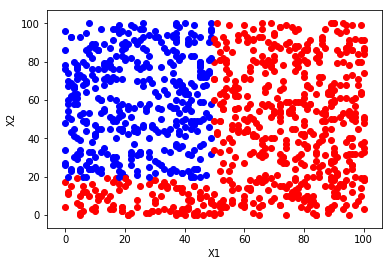
\includegraphics[scale=0.4]{decision_tree_example_data} & \raisebox{.4\height}{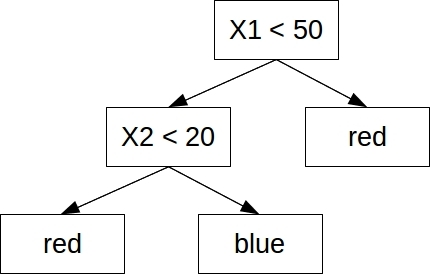
\includegraphics[scale=0.4]{decision_tree_example}}
        \end{tabular}
    \end{center}
    \caption{\label{tab:DecisionTreeExample}Example of Decision Tree}
\end{table}

The algorithms for the construction of decision trees usually work by recursively partitioning the training set $\mathbf{X}$ in such a way that the values of the target vector $\textbf{y}$ are grouped together, until all partitions are composed by a single label. The problem with these building methods is that they produce very complex trees that overfit the training data. Overfitted trees not only lead to poor predictive capabilities on non-training data, but also produce models that can be exceedingly difficult to interpret. A common approach to avoid overfitting in decision trees is to force an early stopping of the algorithm before the tree becomes too complex. Popular stopping criteria include limiting the maximum depth of the tree, requiring a minimum number of sample points at leaf nodes, or computing the accuracy gain yielded by adding new nodes. However, those heuristics demand the optimization of hyperparameters which makes the training process computationally expensive.

    {\color{red} TODO: briefly describe bagging, random forests, and boosting [...] produce multiple trees which are then combined to yield a single consensus prediction [...] combining a large number of trees can often result in dramatic improvement in prediction accuracy, at the expense of some loss of interpretability [...]}

% Subsection: Time Series

\subsection{Time Series Analysis}
\label{sec:intro_time_series}

A time series is a sequence of measurements taken at successively equally spaced points in time, so there exists a natural ordering of the observations. Examples of time series include the daily closing prices of the Standard and Poor's 500 index, the monthly number of passengers of an airline, or the yearly gross domestic product of a country.

\begin{definition}
A \emph{time series} of length $n \in \mathbb{N}$, denoted by $\{ x_t : t=1, \ldots, n \}$ or $\{ x_t \}$, is a sequence $\{ x_1, x_2, \ldots, x_n \}$ of \emph{observed values}.
\end{definition}

The elements $x_i$ of the series correspond to values sampled at fixed time intervals $1, 2, \ldots, n$. The sampling interval must be short enough to provide a very close approximation to the original continuous signal. Observed values could be continuous, discrete or even categorical.

In statistics, a time series is usually represented as a sequence of $n$ random variables, and a particular time series is a realization of this representation. In this sense, $\{ x_t \}$ would denote a collection of random variables. In this book, we do not follow this approach for time series formalization.

Time series forecasting refers to the process of building a model to predict future values of the series based on the previously observed values. Time series forecasting is based on identifying the mean features in data and the random variation, and it is generally based on the assumption that present characteristics will continue in the near future, something that cannot be validated in practice.

\begin{notation}
Given the time time series $\{ x_t : t=1, \ldots, n \}$ we denote $\hat{x}_{t+k \mid t}$ the forecast made at time $t$ for a future value at time $t+k$, where $k$ is the number of steps in the future.
\end{notation}

\subsubsection{Trends and Seasons}

Many time series ... and a repeating seasonal component.

{\color{red} a systematic change in a time series that does not appear to be periodic is known as a trend. [...] A repeating pattern [...] within any fixed period [...] is known as seasonal variation [...] cycles [...] do not correspond to some fixed natural period. [...]}

{\color{red} trend [...] change direction in unpredictable times [...] stochastic trend [...]}

{\color{red} The main features of many time series are trends and seasonal variations that can be modelled deterministically with mathematical functions of time.}

{\color{red} it is usually appropiate to remove trends and seasonal effects before comparing multiple series.}

\begin{definition}
    Let $\{ x_t \}$ be a time series, a \emph{simple additive model} is defined as
    \[
        x_t = m_t + s_t + z_t
    \]
    where $m_t$ is called the \emph{trend component}, $s_t$ is the \emph{seasonal component}, and $z_t$ is the \emph{error term}.
\end{definition}

If the time series presents the property that the seasonal component increases as the trend increases, it might be better to use a multiplicative model.

\begin{definition}
    Let $\{ x_t \}$ be a time series, a \emph{simple multiplicative model} is defined as
    \[
        x_t = m_t \dot s_t + z_t
    \]
    where $m_t$ is called the \emph{trend component}, $s_t$ is the \emph{seasonal component}, and $z_t$ is the \emph{error term}.
\end{definition}

In practice, a simple approach of estimating the trend of a tiem series is to compute a moving average.

\begin{definition}
    Let $\{ x_t \}$ be a time series, a \emph{simple moving average} of lenth $l$ is 
\end{definition}

The best results are achieved when the length $l$ of the moving average is equal to the length of the seasonal component. The seasonal componet can be estimated by

\begin{definition}
    Additive
    \[
        \hat{s}_t = x_t - \hat{m}_t
    \]
    Multiplicative
    \[
        \hat{s}_t = \frac{x_t}{\hat{m}_t}
    \]
\end{definition}


{\color{red} [...] many series are dominated by a trend and/or a seasonal effect [...] A simple additve decomposition model is given by
\[
    x_t = m_t + s_t + z_t
\]
where, a time $t$, $x_t$ is the observed series, $m_t$ is the trend, $_t$ is the seasonal effect, and $z_t$ is an error terms that is, in general, a sequence of correlated random variables with mean zero.

If the seasonal effect tends to increase as the trend increases, a multiplicative model may be more appropriate
\[
    x_t = m_t \dot s_t + z_t
\]

}

\begin{definition}
    
\end{definition}

{\color{red} Once we have identired any trend and seasonal effects, we can deseasonalise the time series and remove the trend. If we use the additive decomposition method, we first calculate the seasonality adjusted time series and then remove the trend by substraction. This leaves the random component, but the random component is not necessarily well modelled by independent random variables. In many cases, consecutive variables will be correlated. If we identify such correlations, we can improve our forecast, quite dramatically if the correlations are high.}

\subsubsection{Second Order Properties}

A possible approach to forecas future values of a time-series based variable is to extrapolate the current trend and to apply some adaptative estimations.


\subsubsection{Exponential Smoothing}

\begin{definition}
Let's $x$ and $y$ two time series. The cross covariance function of $x$ and $y$ as a function of a lag $k$, denoted $\gamma \left( x, y \right)$, is defined as:
\[
    \gamma \left( x, y \right) = E 
\] 

\end{definition}

\begin{definition}

\end{definition}

%
% Autocorrelation, Crosscorrelation and Partial Autocorrelation
% 
\subsubsection{Autocorrelation, Cross-correlation and Partial Autocorrelation}
\label{sub:autocorrelation}

{\color{red} Another important feature of most time series is that observations close toghether in time tend to be correlated (serially dependent)}

{\color{red} two unrelated time series will be correlated if they both contain a trend}

Autocorrelation measures the (Pearson) correlation of a time series with a delayed version of itself, and as a function of that delay. Autocorrelation is intended to estimate the degree of similarity of an observation with respect to previous observations.

\begin{definition}
Let $\{\mathbf{X}_t\}$ be a time series with mean $\mu$ and varianze $\sigma^2$. The \emph{autocorrelation} function, denoted by $\rho$, is defined as:
\[
\rho_x(k) = \frac{E\left[\left(x_{t}-\mu\right)\left(x_{t+k}-\mu\right)\right]}{\sigma^{2}}
\]
The value $k$ is called \emph{lag}.
\end{definition}

The autocorrelation function is not defined for all time series, because the mean may not exist (time series with a trend), or the variance may be zero (constant time series). A time series for which the autocorrelation is defined is called \emph{second order stationary}.

The \emph{sample autocorrelation} is computed in practice by:
\[
\hat{\rho}_x(k) = \frac{ \frac{1}{n}\sum_{t=1}^{n-k}\left(x_{t}-\bar{x}\right)\left(x_{t+k}-\bar{x}\right) }{ \left( \frac{1}{n}\sum_{t=1}^{n}\left(x_{t}-\bar{x}\right) \right)^2 }
\]
On the contrary of what happened with autocorrelation, sample autocorrelation is defined in case of time series with a trend. However, we must be carefull about the interpretation of the results. In general, sample autocorrelation is applied over the residuals of a time series once the trend and the seasonal components have been removed.

A correlogram is a plot of the sample autocorrelations $\hat{\rho}(k)$ versus time lags $k$ (see Figure {\color{red} XXX}). The dotted lines are drawn at $-\frac{1}{n}\pm\frac{2}{\sqrt{n}}$. If $\hat{\rho}(k)$ is outside these lines for a value of $k$ we have evidence against the null hypothesis that $\hat{\rho}(k)=0$ at the $5\%$ level (See Section {\color{red} XXX}). It is expected that $5\%$ of the estimates $\hat{\rho}(k)$ fall outside these lines.

\begin{example}
{\color {red} TODO: Insert Figure. If the example is drawn using matplotlib.pyplot.acorr, the above paragraph is not true. Investigate how the shared areas in the correlogram used by matplotlib are computed.}
\end{example}

Crosscorrelation measures ...

\begin{definition}
Let $\{\mathbf{x}_t\}$ and $\{\mathbf{y}_t\}$ be time series with means $\mu_x$ and $\mu_y$ and variances $\sigma_x^2$ and $\sigma_y^2$. The \emph{crosscorrelation} function, denoted by $\rho$, is defined as:
\[
\rho_{x,y}(k) = \frac{E\left[\left(x_{t+k}-\mu_x\right)\left(y_t-\mu_y\right)\right]}{\sigma_x \sigma_y}
\]
The value $k$ is called \emph{lag}.
\end{definition}

If the crosscorrelation is defined it is said that the combined model is \emph{second order stationary}.

The \emph{sample crosscorrelation} is computed in practice by:
\[
\hat{\rho}_{x,y}(k) = \frac{ \frac{1}{n}\sum_{t=1}^{n-k}\left(x_{t}-\bar{x}\right)\left(y_{t+k}-\bar{y}\right) }{ \frac{1}{n}\sum_{t=1}^{n}\left(x_{t}-\bar{x}\right) \frac{1}{n}\sum_{t=1}^{n}\left(y_{t}-\bar{y}\right) }
\]

In general, sample crosscorrelation is applied over the residuals of both time series once trends and the seasonal components have been removed.

In the same way we draw a correlogram we can plot a crosscorrelogram of the crosscorrelation between to time series.

\begin{example}
{\color {red} TODO: Insert Figure. If the example is drawn using matplotlib.pyplot.acorr, the above paragraph is not true. Investigate how the shared areas in the correlogram used by matplotlib are computed.}
\end{example}


% Structural Time Series
\subsubsection{Structural Time Series}

{\color{red} A univariate structural time series model is one which is formulated in terms of components which, although unobservable, have a direct interpretation. It not only provides the basis for making predictions of future observations, but it also provides a description of the salient features of a time series.}

Examples of structural components could be a trend, a seasonal effect, a cycle, an intervention, or the noise.

\begin{definition}
Let $\mathbf{x}_t$ be a time series. The structural decomposition of $\mathbf{x}_t$ in given by
\[
y_t = \mu_t + \psi_t + \gamma_t + \ldots + \varepsilon_t
\]
where $\mu_t, \psi_t, \gamma_t, \ldots$ is a finite collection of additive stochastic terms, called structural components, and $\varepsilon_t$ is a random term composed by independent and identically distributed samples with zero mean. 
\end{definition}

\begin{example}
dd
\end{example}

\subsubsection{State Space Model}

\begin{definition}
Let $y_t$ be a time series. The state space decomposition of $y_t$ is given by
\begin{align*}
    & y_t          \quad = \mathbf{Z}_t \alpha_t + \epsilon_t \\
    & \alpha_{t+1} \quad = \mathbf{T}_t \alpha_t + \mathbf{R}_t \eta_t
\end{align*}
where
\begin{align*}
    & \alpha_t     \quad explain \\
    & \mathbf{Z}_t \quad explain \\
    & \mathbf{T}_t \quad explain
\end{align*}

\begin{equation}
    \label{eq:measurement_equation}
    \mathbf{y} = f\left( \mathbf{X} \right) + \epsilon
\end{equation}

measurement equation and transition equation

\end{definition}

% Multivariate Time Series
\subsubsection{Mulivariate Time Series}

{\color{red} TODO: Introduce this section.}

A time series could be multivariate, where a dependant variable $\{ x_{m+1} \}$ is sampled toghether with a collection of $m$ independent variables $\{ \mathbf{x}_i \}$.

\begin{definition}
A \emph{multivariate time series} of length $n \in \mathbb{N}$ composed by $m+1 \in \mathbb{N}$ variables, denoted by $\{ \mathbf{x}^i_t : i=1, \ldots, m+1 \; \text{and} \; t=1, \ldots, n\}$ or $\{ \mathbf{x}_t \}$, is a sequence $\{ \mathbf{x}_1, \mathbf{x}_2, \ldots, \mathbf{x}_n \}$ of \emph{observed vector values}. The time series $\{ \mathbf{x}^{m+1} \}$ is called the \emph{independent variable}, and the time series $\{ \mathbf{x}^i : i=1, \ldots m\}$ the \emph{dependant variables}.
\end{definition}

{\color{red} TODO: cross-correlation and partial cross-correlation.}

%
% Minimum Message Length
%
\section{Minimum Message Length}
\label{sec:MML}

The \emph{Minimum Message Length} (MML) is based on the idea that a good theory, or explanation, for a dataset is a small collection of premises under which the data is not surprising. The best theories are those which are short, able to explain most of the data, and with a high accuracy. An \emph{explanation message} is composed by two parts: the fist part comprises all the premises induced from the data, including numerical values; the second part contains all the data that cannot be derived from the premises. The message also assumes the existence of some already known and accepted premises (prior knowledge). Given the prior premises and the message it should be possible to recover the original dataset. According to the MML, theories are not rejected due to contradictory measurements, they only make the second part of the message longer.

In the MML principle, a message is a lossless encoded version of the original data. The first part of the message contains a probabilistic model about the data, and the second part is the data encoded using this model. We are interested in finding the shortest possible explanation message. If the length of the explanation message is longer than the original data, the theory is considered unacceptable.

Bayes' theorem (see Theorem \ref{th:bayes}) states that the probability $P(H \mid E)$ of a hypothesis $H$ given an evidence $E$ is:
\[
    P(H \mid E) = \frac{ P( E \mid H ) P(H) }{ P(E) }
\]
We are interested in finding the hypothesis $H$ with the highest posterior probability $P(H \mid E)$ of being true, assuming a fixed evidence $E$. That is, we are looking for maximize $P( E \mid H ) P(H)$ or, equivalently, maximize $P ( H \wedge E )$.

The \emph{Minimum Message Length} principle (MML for short) is based on the idea that the length of encoding $H \wedge E$ as a binary string using an optimal code is equal to $- \log_2 P ( H \wedge E )$ (see Theorem \ref{th:optimal_codes}). That is:
\[
    l(H \wedge E) = - \log_2 P ( H \wedge E ) = - \log_2 P( E \mid H ) P(H) = - \log_2 P( E \mid H ) - \log_2 P(H)
\]
The most probable model $H$ would be that model that allows us to encode $H \wedge E$ with the shortest possible string. The encoded string would be composed by two parts, a general assertion about the data, and a detailed description of the data assuming that the assertion is true.

Let $\mathbb{X}$ be a discrete set composed by all possible datasets, $\mathcal{X}$ a random variable taking values on $\mathbb{X}$, and $f(X \mid \theta)$ a probability distribution for $\mathcal{X}$ given the parameter $\theta$.

\begin{definition}
    Let $\Theta$ be a discrete set of possibles parameters for $f$ with probability distribution $h(\theta) \, \theta \in \Theta$, and let $\hat\theta \in \Theta$ be an inferred parameter. An \emph{assertion} is the encoded version of $\hat\theta$ using an optimal code given the probability distribution $h$.
\end{definition}

The length of the assertion given an optimal binary code is $- \log_2 h(\hat\theta)$ (see Section {\ref{sec:Optimal-Codes}). Note that $\theta$ could be a single scalar or a vector of values. Moreover, $\theta$ could be related to more than one family of probability distributions $f$.

\begin{definition}
    Let $X \in \mathbb{X}$ be a dataset, and $\hat \theta \in \Theta$ an inferred value for the distribution $f$. A \emph{detail} is the encoded version of $X$ using an optimal code given the probability distribution $f(X \mid \hat\theta)$.
\end{definition}

The length of the detail given an optimal binary code is $- \log_2 f( X \mid \hat\theta )$. That is, the length of the detail is the negative of the log-likelihood of $X$ given $\hat\theta$.

\begin{definition}
    Let $X \in \mathbb{X}$ be a dataset, and $\hat \theta \in \Theta$ an inferred value for the distribution $f$ A \emph{message} for the dataset $X$ given an inference $\hat\theta \in \Theta$ is the concatenation of the assertion for $\hat\theta$ and the corresponding detail for $X$ given $\theta$.
\end{definition}

The length of a message given an optimal binary code is $- \log_2 h \left( \hat\theta \right) - \log_2 f \left( X \mid \hat\theta \right)$. The length of a message allow us, for example, to compare the posterior probabilities of two competing explanations or hypotheses $\hat\theta_1$ and $\hat\theta_2$.

\begin{definition}
    Let $X \in \mathbb{X}$ be a dataset. The \emph{Minimum Message Length} of $X$, denoted by $MML(X)$, is given by:
    \[
        MML(X) = \argmin_{\hat\theta \in \Theta} \left( - \log_2 h \left( \hat\theta \right) - \log_2 f \left( X \mid \hat\theta \right) \right)
    \]

\end{definition}

In practice, the actual messages will not be constructed, since our interest is in the length of the messages, not in their content. It is assumed that the sets $\mathbb{X}$ and $\Theta$ and the functions $f(X \mid \hat\theta)$ and $h(\theta)$ are known a priori, and so, it is not necessary to include them as part of our encoding message.

\begin{example}
    \label{ex:MML}
    Consider an experiment in which we toss a weighted coin $100$ times. Denote by $1$ if we get a face and $0$ a cross, so that each experiment is a binary string of length $100$. Our collection of all possible datasets is $\mathbb{X} = \mathcal{B}^{100}$, $\theta$ is a number in the interval $[0, 1]$, the likelihood $f (X \mid \theta)$ follows a binomial distribution (that is, $f (X \mid \theta) ) = \theta^n (1-\theta)^{100-n}$ where $n$ is the number of faces in $X$), and since we do not know anything about how the coin is weighted, we could assume that $h(\theta)$ is the uniform distribution in the interval $[0, 1]$ (that is, $h(\theta) = 1$ for $\theta \in \Theta$). Under these assumptions, the length of a message for $X$ given an inferred parameter $\hat\theta$ would be:
    \[
        - \log_2 h \left( \hat\theta \right) - \log_2 f \left( X \mid \hat\theta \right) = - n \log_2 \hat\theta - (100-n) \log_2 (1 - \hat\theta)
    \]
    We are interested in finding the value of $\hat\theta$ that minimizes the length of the encoded version of $X$, that is, the minimum message length for $X$.
\end{example}

A Maximum A Posteriori analysis of the experiment in Example \ref{ex:MML} would provide the same inference for $\hat\theta$ than the Minimum Message Length approach. Moreover, given that $h(\theta)$ follows an uniform distribution, a Maximum Likelihood approach would reach exactly the same value for $\hat\theta$.

%
% Minimum Description Length
%
\section{Minimum Description Length}
\label{sec:MDL}

The \emph{Minimum Description Length} (MDL) principle is a reformulation
of the Kolmogorov complexity with the goal to make it applicable to
solve practical problems. MDL explicitly address the two most important
practical limitations of the Kolmogorov complexity: its uncomputability
(in general, the Kolmogorov complexity cannot be computed), and the
large constants involved in the invariance theorem (that makes it
inapplicable to short strings). The approach of MDL to these problems
is to scale down Kolmogorov complexity until it does become applicable:
instead of using general-purpose computer languages, MDL is based
on fixed languages and coding functions.

In contrast to Kolmogorov that states that the complexity of a string
is equal to the length of the shortest program that prints that string,
MDL proposes that our capacity to learn about a string is equivalent
to our ability to compress that string. The idea behind MDL is to
describe a dataset with the help of an hypothesis: the more the hypothesis
fits the data (and here good fit equals learning), the more we can
compress the data given that hypothesis.

In our particular case, we are interested in MDL because it will allow
us to compute the nescience of a topic given a dataset, instead of
requiring a text describing the topic. Thus, given a topic $t$ and
a sample dataset $D=\left\{ x_{1},x_{2},\ldots,x_{n}\right\} $, the
nescience of a particular hypothesis $H$ will be related to the capacity
of that hypothesis to compress the dataset.

MDL comes into two versions, \emph{simplified (two-part code) MDL}
and \emph{refined MDL}. Simplified MDL is easier to understand, and
it will allows us to introduce some important concepts and notation.
The extension of the concept of nescience to datasets will be based
on the refined version of MDL.


    {\color{red} TODO: Explain how this relates to cross entropy}


In this section we are going to introduce the two-part code version
of the minimum description length principle for probabilistic models.

\emph{Given a set of candidate models (a set of probability distributions
    (for example first-order Markov chains) or functions of the same functional
    form (for example the kth degree polynomials)) $\mathcal{H^{\left(\text{1}\right)}},\mathcal{H}^{\left(2\right)},\ldots$
    the simplified,} \emph{two-part version,} \emph{of the} Minimum Description
Length Principle \cite{Gr=0000FC05}\emph{ states that the best point
    hypothesis (a single probability distribution (e.g. a Markov chain
    will all parameters values specified) $H\in\mathcal{H^{\left(\text{1}\right)}}\cup\mathcal{H}^{\left(2\right)}\cup\ldots$
    to explain the data $D=\left(x_{1},\ldots,x_{n}\right)\in\mathcal{X}^{n}$
    is the one that minimizes the sum $L(M)+L(D\mid M)$, where $L(M)$
    is the length (in bits) of the model description, and $L(D\mid M)$
    is the length (in bits) of the data encoded with the help of the hypothesis
    ... there is only one reasonable choice for this code ... the so-called
    Shannon-Fano code ... Each hypothesis $H$ may be viewed as a probability
    distribution over $\mathcal{X}^{n}$. For each such distribution there
    exists a code with length function $L$ such that for all $x^{n}\in\mathcal{X}^{n}$
    we have that $L\left(x^{n}\right)=-\log_{2}P\left(x^{n}\mid H\right)$.
    The quantity $L(M)$ depends on each model.}

\emph{A description of the data ``with the help of'' a hypothesis
    means that the better the hypothesis fits the data, the shorter the
    description will be. A hypothesis that fits the data well gives us
    a lot of information about the data. Such information can always be
    used to compress the data. This is because we only have to code the
    errors the hypothesis makes on the data rather than the full data.}

\emph{The sum of the two description length will be minimized at a
    hypothesis that is quite (but not too) ``simple'', with a good (but
    not perfect) fit.}

The length of the data given the model, that is, \emph{$L(D\mid M)$.}

\[
    -\log P(D)=L_{C}(D)
\]


This choice for C gives a short codelegth to sequences which have
high probability according to (k, ttita) while it gives a high codelength
to sequences with low probability. The codelength thus directly reflects
the goodness-of-fit of the data with respect to (k,tita) measured
in terms of the probability fo D according to (k,tita).

When we say we ``code the data D with the help of probabilistic hypothesis
P'' we mean that we code D using the Shannon-Fano code corresponding
to P.

\[
    L(D\mid P):=-\log P(D)
\]


the code with these lengths is the only one that would be optimal
if P where true. (mention we are only interested in code lengths,
we are not interested in to find the code itself).

For \emph{$L(M)$ we use the standard code for integers.}

\begin{example}
    Markov Chain Hypothesis Selection: Suppose we are given data $D X\textasciicircum{}n$
    where $X=\{0,1\}$. We seek a reasonable model for D that allows us to
    make good predictions of future data coming from the same source.
    We decide to model our data using the cass B o all Markov chains ${[}...{]}$
    we face the problem of overfitting: for a given sequence $D=(x1,...,xn)$,
    there may be a Markov chain P of very high order that fits data D
    quite well but that will behave very badly when predicting future
    data from the same source.
\end{example}

\subsection{Refined MDL}

\emph{In refined MDL, we associate a code for encoding $D$ not with
    a single $H\in\mathcal{H}$ but with the full model $\mathcal{H}$
    ... we design a single one-part code with lengths $\bar{L}\left(D\mid H\right)$
    (called the stochastic complexity of the data given the model). This
    code is designed such that whenever there is a member of (parameter
    in) $\mathcal{H}$ that fits the data well, in the sense the $L\left(D\mid H\right)$
    is small, then the codelenth $\bar{L}\left(D\mid H\right)$ will also
    be small. Codes with this property are called universal codes.}

\emph{There are at least four types of universal codes:}
\begin{enumerate}
    \item \emph{The normalized maximum likelihood (NML) code and its variations.}
    \item \emph{The Bayesian mixture code and its variations.}
    \item \emph{The prequential plug-in code.}
    \item \emph{The two-part code.}
\end{enumerate}
\emph{Refined MDL is a general theory of inductive inference based
    on universal codes that are designed to be minimax, or close to minimax
    optimal. It has mostly been developed for model selection, estimation
    and prediction.}

%
% Section: Multiobjective Optimization
%

\section{Multiobjective Optimization}
\label{sec:multiobjective_optimization}

Multiobjective optimization is the area of mathematics that deals with the problem of simultaneously optimizing two or more conflicting functions. Multiobjective optimization has been applied in many areas of science, including engineering, economics and logistics, where there is no single solution that simultaneously satisfies all objectives, so a decision must be made in the presence of trade-offs between the conflicting goals.

From a formal point of view, we are interested in solving the following \emph{multiobjective optimization} problem:
\begin{align*}
     & \text{minimize}	  \quad \left\{f_1(\mathbf{x}), f_2(\mathbf{x}), \ldots, f_k(\mathbf{x}) \right\} \\
     & \text{subject\;to} \quad \mathbf{x} \in \mathbf{S}
\end{align*}
where $f_i:\mathbb{R}^n \rightarrow \mathbb{R}$, $i = 1, \ldots, k$, are two or more objective \emph{objective functions}, and the nonempty set $\mathbf{S} \subset \mathbb{R}^n$ is the \emph{feasible region}, whose elements $\mathbf{x} = \left( x_1, x_2, \ldots, x_n \right)$ are \emph{decision vectors}. The image of the feasible region $f(\mathbf{S}) \subset \mathbb{R}^k$, denoted by $\mathbf{Z}$, is called \emph{objective region}, and its elements $\mathbf{z} = \left(f_1(\mathbf{x}), f_2(\mathbf{x}), \ldots, f_k(\mathbf{x}) \right)$ \emph{objective vectors}. In some applications, the feasible region is formed by a collection of inequality constraints $\mathbf{S} = \{ \mathbf{x} \in \mathbb{R}^n \mid g(\mathbf{x}) = \left( g_1(\mathbf{x}), \ldots, g_m(\mathbf{x}) \right) \leq 0 \}$.

In this book we will be dealing with nonlinear multiobjective minimization problems, where at at least one of the objective functions, or the constraint functions, is not linear. Objective functions can be also incommensurable, that is, measured in different units or in different scales.

Since the objective functions are conflicting, it does not exist a single solution that is optimal with respect to every objective function (the objective region is partially ordered). 

\begin{definition}
A decision vector $\mathbf{x} \in \mathbf{S}$ \emph{dominates} another decision vector $\mathbf{y} \in \mathbf{S}$ if $f_i(\mathbf{y}) \leq f_i(\mathbf{x})$ for all $i \in \{1, \ldots, k\}$ and $f_j(\mathbf{y}) < f_j(\mathbf{x})$ for at least one $j \in \{1, \ldots, k\}$. An objective vector $\mathbf{z} \in \mathbf{Z}$ \emph{dominates} another objective vector $\mathbf{w} \in \mathbf{Z}$ if $w_i \leq z_i$ for all $i \in \{1, \ldots, k\}$ and $w_j < z_j$ for at least one $j \in \{1, \ldots, k\}$.
\end{definition}

Dominance can be studied from the point of view of decision variable space or objective space. An objective vector dominates another objective vector if, and only if, its corresponding decision vector also dominates the other decision vector.

We are interested in those objective vectors for which none of its individual components can be improved without deteriorating at least one of the others.

\begin{definition}
\label{def:pareto_optimal}
A decision vector $\mathbf{x} \in \mathbf{S}$ is \emph{Pareto optimal} if there does not exists another decision vector $\mathbf{y} \in \mathbf{S}$ such that $\mathbf{y}$ dominates $\mathbf{x}$. An objective vector $\mathbf{z} \in \mathbf{Z}$ is Pareto optimal if there does not exits another objective vector $\mathbf{w} \in \mathbf{Z}$ such that $\mathbf{w}$ dominates $\mathbf{z}$.
\end{definition}

Pareto optimality can be also studied from the point of view of decision variable space or objective space. An objective vector is Pareto optimal if, and only if, its corresponding decision vector is Pareto optimal.

\begin{definition}
The set of Pareto optimal solutions, denoted by $\mathbf{P}_D$, is called the \emph{Pareto optiomal set}. The set of Pareto optimal solutions in the space of objectives, denoted by $\mathbf{P}_O$, is called the \emph{Pareto frontier}.
\end{definition}

Sometimes, in practice, it is convenient to use a more restrictive definition of the concept of optimaily, in which we identify those vectors for which there does not exist any other vector that improves over all the components simultaneously.

\begin{definition}
A decision vector $\mathbf{x} \in \mathbf{S}$ is \emph{weakly Pareto optimal} if there does not exist another decision vector $\mathbf{y} \in \mathbf{S}$ such that $f_i ( \mathbf{y} ) < f_i ( \mathbf{x} )$ for all $i = 1, \ldots, k$. An objective vector $\mathbf{z} \in \mathbf{Z}$ is weakly Pareto optimal if there does not exists another objective vector $\mathbf{w} \in \mathbf{Z}$ such that $w_i < z_i$ for all $i = 1, \ldots, k$.
\end{definition}

An objetive vector is weakly Pareto optimal if its corresponding decision vector is weakly Pareto optimal. Oviously, the Pareto optimal set is a subset of the weakly Pareto optimal set.

\begin{example}
\label{ex:pareto}
\begin{figure}[h]
\centering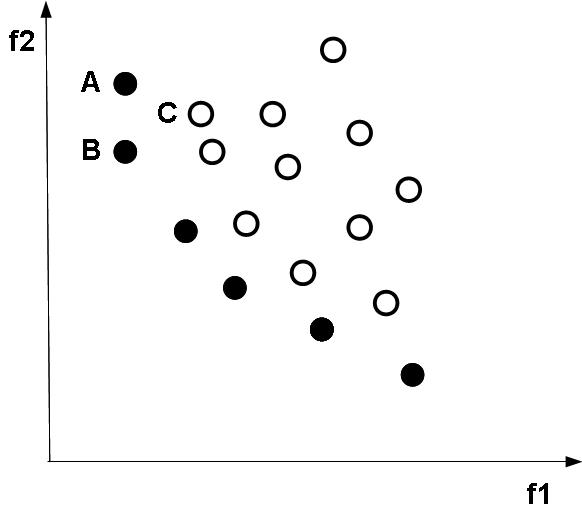
\includegraphics[scale=0.3]{pareto.jpg}
\caption{\label{fig:pareto}Pareto optimality.}
\end{figure}
{\color{red} TODO: Provide an example based on a multi-variable function.} In figure \ref{fig:pareto} we have depicted a sample of the objective region of a multiobjetive optimization problem composed by two real-valued objective functions $f_1$ and $f_2$ that we are interested in minimizing. White points are not weakly Pareto optimal since there exist points that improve both components at the same time (for example, point $\mathbf{B}$ improves point $\mathbf{C}$ in both functions). Black points are weakly Pareto optimal since there is no point that improves both components at the same time. Point $\mathbf{A}$ is not Pareto optimal since point $\mathbf{B}$ improves one component without deteriorating the other.
\end{example}

Mathematically speaking all the solutions that compose the Pareto optimal set are equally good. However, for the majority of the practical applications, it is highly desirable to have a single solution. Finding this solution requires additional information not included in the definition of the optimization problem. The relation of preference between objective function values is expresed using a \emph{decision maker}, that it is supposed to have additional insights about the problem to solve. In this sense, solving a multiobjective optimization problem would require to find those feasible decision vectors that it are Pareto optimal and that satisfy the additional requirements imposed by the decision maker.

In practice, we assume that the preferences of the decision maker can be expressed using a value function.

\begin{definition}
A \emph{value function} is a function $U : \mathbb{R}^k \rightarrow \mathbb{R}$ that assigns t each objective vector $\mathbf{z} = \left( z_1, \ldots, z_k \right)$ a single real value $U(\mathbf{z})$.
\end{definition}

{\color{red} value functions are miximized}

Value functions allow us to order the vectors of the objective region $\mathbf{Z}$. We are interested in applying the value function to the Pareto optimal subset to find a unique solution to the multiobjective optimization problem.

% Subsection: Range of the Solutions

\subsection{Range of the Solutions}
\label{sec:range_solutions}

We are intersted in investigating the range of the solutions included in the Pareto optimal set. To do that, we have to find the lower and upper bounds of this set. In the rest of this section, we assume that the objective functions are bounded over the feasible region $\mathbf{S}$.

{\color{red} TODO: rewrite the concepts of nadir and ideal vector using the supremum and infimum.}

An objective vector that minimizes all objective functions is called an ideal objective vector.

\begin{definition}
A vector $\mathbf{z}^\star \in \mathbb{R}^k$ is called \emph{ideal} if each of its components $z_i$, minimizes the objective funcion $f_i \left( \mathbf{x} \right)$ subject that $\mathbf{x} \in \mathbf{S}$.
\end{definition}

If there exits an ideal objective vector that belongs to the feasible region, that is $\mathbf{z}^\star \in \mathbf{Z}$, then that vector would be a solution of the optimization problem, and that solution would be unique. Ideal vectors are lower bounds to the Pareto set.

The upper bound of the Pareto optimal set is given by the nadir objective vector. The nadir vector can be estimated using the decision vectors calculated when obtaining the objective ideal vector.

\begin{definition}
Let $\mathbf{z}^\star \in \mathbb{R}^k$ be an ideal objective vector. The set of decision vectors $\{ \mathbf{x}^\star_1, \ldots, \mathbf{x}^\star_k \}$ used to compute $\mathbf{z}^\star$ is called the \emph{payoff table} for $\mathbf{z}^\star$. That is, if $\mathbf{z}^\star = \{ z^\star_1, \ldots, z^\star_k \}$, we have that $z^\star_i = f_i \left( \mathbf{x}^\star_i \right)$.
\end{definition} 

It turns out that $f_i \left( \mathbf{x}^\star_i \right)$ ($i = 1, \ldots, k$) is minimal for all for all the elements of the payoff table.

Having the payoff table we can provide an estimation for the nadir vector. For simplicity, let's $f^\star_{ij}$ denote the value of the objective function $f_i$ computed over the vector $\mathbf{x}^\star_j$, where $i, j = 1, \ldots, k$.

\begin{definition}
Let $\mathbf{z}^\star \in \mathbb{R}^k$ be an ideal objective vector, and $\{ \mathbf{x}^\star_1, \ldots, \mathbf{x}^\star_k \}$ its payoff table. The \emph{nadir} objective vector $\mathbf{z}^{nad} = \{ z^{nad}_1, \ldots, z^{nad}_k \}$ is given by $z^{nad}_i = \max_j f^\star_{ij}$.
\end{definition}

The ideal objective vector and the nadir objective vector may, or may not, be feasible. In figure \ref{fig:nadir} are depicted the ideal (vector $\mathbf{E}$) and nadir (vector $\mathbf{F}$) vectors of the multiobjective optimization problem of Example \ref{ex:pareto}.

\begin{figure}[h]
\centering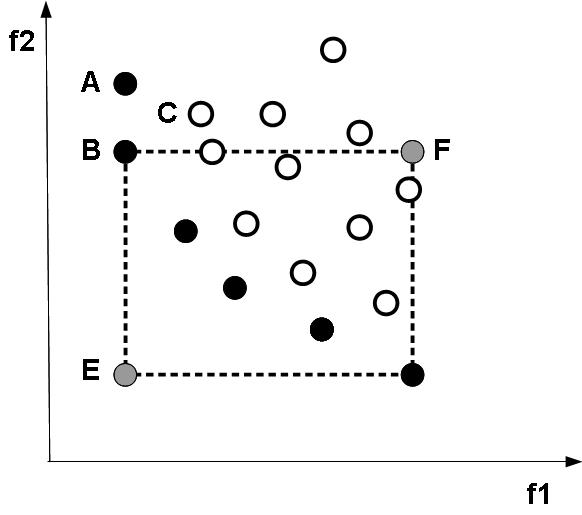
\includegraphics[scale=0.3]{nadir.jpg}
\caption{\label{fig:nadir}Ideal and Nadir vectors.}
\end{figure}

For some applications, the range of values of the objective functions can differ by orders of magnitude. In those situations, it is advisable to normalize them, so the values are in the same scale. We can use the ideal and nadir vector for this normalization process, by replacing each objective function $f_i (\mathbf{x}) (i = 1, \ldots, k)$ by the normalized function
\[
\frac{f_i(\mathbf{x}) - z^\star_i}{z^{nad}_i - z^\star_i}
\]

% Subsection: Trade-offs

\subsection{Trade-offs}
\label{sec:trade_offs}

Since the functions we want to minimize are conflicting, sometimes we have to assume that the only way to gain a benefit in on aspect of the problem is to losse something in another aspect. How much we have to give up in one objective to improve a certain quantity in the other is called a trade-off.

\begin{definition}
Let $\mathbf{x}^1, \mathbf{x}^2 \in \mathbf{S}$ be two decision vectors. The \emph{ratio of change} between the functions $f_i$ and $f_j$ for the vectors $\mathbf{x}^1, \mathbf{x}^2$, denoted by $\Delta_{ij}$, is defined as:
\[
\Delta_{ij} ( \mathbf{x}^1, \mathbf{x}^2 ) = \frac{f_i(\mathbf{x}^1) - f_i(\mathbf{x}^2)}{f_j(\mathbf{x}^1) - f_j(\mathbf{x}^2)}
\] 
for all $i, j = 1, \ldots, k$ such that $f_j(\mathbf{x}^1) - f_j(\mathbf{x}^2) \neq 0$.
\end{definition}

$\Delta_{ij}$ is called a \emph{partial trade-off}, involving $f_i$ and $f_j$ between $\mathbf{x}^1$ and $\mathbf{x}^2$ if $f_l(\mathbf{x}^1) = f_l(\mathbf{x}^2)$ for all $l = 1, \ldots, k$, $l \neq i, j$. If $f_l(\mathbf{x}^1) \neq f_l(\mathbf{x}^2)$ for at least one $l = 1, \ldots, k$, and $l \neq i, j$ then $\Delta_{ij}$ is called a \emph{total trade-off}.

If the trade-off between two objective functions is very small or very large, that is, if a small change in one aspect of the optimization problem has a significant impact in another aspect, we have a case that is similar to having a weakly Pareto solution that it is not Pareto optimal. In some practical applications is convenient to filter out those solutions that present this undesirable behaviour.

\begin{definition}
A decision vector $\mathbf{x} \in \mathbf{S}$ is \emph{properly Pareto optimal} if it is Pareto optimal and if there exists a real number $M > 0$ such that for each $f_i$ and $\mathbf{y} \in \mathbf{S}$ satisfying $f_i ( \mathbf{y} ) < f_i ( \mathbf{x} )$, there exists at least one $f_j$ such that $f_j ( \mathbf{x} ) < f_j ( \mathbf{y} )$ and
\[
\frac{f_i ( \mathbf{x} ) - f_i ( \mathbf{y} )}{f_j ( \mathbf{y} ) - f_j ( \mathbf{x} )} \leq M
\]
An objective vector $\mathbf{z} \in \mathbf{Z}$ is properly Pareto optimal if the decision vector corresponding to it is properly Pareto optimal.
\end{definition}

A solution is properly Pareto optimal if there is at least one pair of objectives functions for which a small decrement in one objective is possible only at the expense of a large increment in the other objective.

Note that the properly Pareto optimal set is a subset of the Pareto optimal set, and the Pareto optimal set is a subset of the weakly Pareto optimal set.

% Optimization Methods

\subsection{Optimization Methods}

{\color{red} Generating Pareto optimal solutions plays an important role in multiobjective optimizatoin, and mathematically the problem is considered to be solved when the Pareto optimal set is found [...] However, this is not always enough. We want to obtain only one solution. This means that we must find a way to put the Pareto optimal solutions in a comple order. This is why we need a decision maker an his preference structure.}

{\color{red} In general, multiobjective optimization problems are solved by scalarization [...] scalarization means converting the problem into a single or a family of single objective optimization problems with a real-valued objective function}

{\color{red} three requirement are set for a scalarization function: 1)  It can cover any Pareto optimal solution. 2) Every solution is Pareto optimal.}

{\color{red} [...] classify the methods according to the participation of the decision maker in the solution process. The classes are: 1) methods where no articulation of preference information is used (no-preference methods) 2) methods where a posteriory articulation of preference is used (a posteriory methods) 3) methods whre a priori articulation of preference information is used (a priory methods), and 4) methods whre progressive articulation of preference information is used (interactive methods).}

In no-preference methods, the knowledge of the decision maker is not taken into account, and the optimization problem is solved using a relatively simple method. In a posteriory methods, the set (or part of it) of Pareto optimal points is identified and then the decision maker select the preferred solution among the alternatives.

\subsubsection{Global Criterion}
\label{sub:multiobjective_global_criterion}

The global criterion is a non-prefrence method in which the distance between some reference point and the fasible objective region is minimized. In this method, all the objective functions are considered to be equally important. As reference point it is usually used the ideal vector, and as metric it is common to use a $L_p$-metric. Under these assumptions, the goblal criterion method becomes the following minimization problem:
\begin{align*}
     & \text{minimize}    \quad \left( \sum_{i=1}^k \left( f_i(\mathbf{x}) - z_i^\star \right)^p \right)^{\frac{1}{p}} \\
     & \text{subject\;to} \quad \mathbf{x} \in \mathbf{S}
\end{align*}
Different values for $p$ result in different solutions to the minimization problem. Common values for $p$ are $1$, $2$ or $\infty$. 

\begin{proposition}
\label{prop:global_criterion_pareto_optimal}
The solution of the $L_p$-based global criterion is Pareto optimal.
\end{proposition}
\begin{proof}
Let $\mathbf{x}$ be a solution of the $L_p$-based global criterion problem, with $1 \leq p < \infty$, and assume that $\mathbf{x}$ is not Pareto optimal. Then, according to Definition \ref{def:pareto_optimal} there must exists a point $\mathbf{y} \in \mathbf{S}$ such that $f_i( \mathbf{y} ) \leq f_i( \mathbf{x} )$ for all $i = 1, \ldots, k$, and $f_j( \mathbf{y} ) < f_j( \mathbf{x} )$ for at least one $j$. Then we have that $( f_i(\mathbf{y}) - z_i^\star )^p \leq ( f_i(\mathbf{x}) - z_i^\star )^p$ for all $i \neq j$ and $( f_j(\mathbf{y}) - z_j^\star )^p < ( f_j(\mathbf{x}) - z^\star )^p$. Adding all these terms and raising to the $1/p$ power, we obtain
\[
\left( \sum_{i=1}^k \left( f_i(\mathbf{y}) - z_i^\star \right)^p \right)^{\frac{1}{p}} < \left( \sum_{i=1}^k \left( f_i(\mathbf{x}) - z_i^\star \right)^p \right)^{\frac{1}{p}} 
\]
which is a contradiction with the fact that $\mathbf{x}$ is a solution to the minimization problem.
\end{proof}

Although all the solutions selected by the $L_p$-based global criterion are Pareto optimal, as we have proved in previous proposition, there are solutions of the optimal Pareto set are that will never be selected by this method. In practice it is convenient to normalize the range of the objective values, so that those points closer to the ideal vector do not receives more importance. A common normalization term used in practice is $z_i^{nad} - z_i^\star$.

\subsubsection{Weighting Method}

{\color{red} The weighting method is a simple way to generate different Pareto optimal solutions.}

{\color{red} In the weighting method [...] the idea is to associate each objective function with a weighting coefficient and minimize the weighted sum of the objectives. In this way, the multiple objective functions are transformed into a single objective function. We suppose that the weighting coefficients $w_i$ are real numbers such that $w_i \geq 0$ for all $i = 1, \ldots, k$. It is also usually supposed that the weights are normalized, that is $\sum_{i=1}^k w_i = 1$.}

{\color{red} The multiobjective optimization problem is modified into the following problem, to be called a weighting problem:}
\begin{align*}
     & \text{minimize}    \quad \sum_{i=1}^k  w_i  f_i(\mathbf{x}) \\
     & \text{subject\;to} \quad \mathbf{x} \in \mathbf{S}
\end{align*}
{\color{red} where $w_i \geq 0$ for all $i = 1, \ldots, k$ and $\sum_{i=1}^k w_i = 1$.}

{\color{red} [...] weighting coefficient zero makes no sense. It means that we hae included in the problem some objective function that has no significance at all.}

{\color{red} The objective functions should be normalized or scaled so that their objective values are approximately of the same magnitude [...] Only in this way can one control and manoeuvre the method to produce solutions of a desirable nature in proportion to the ranges of the objective functions. Otherwise the role of the weighting coefficients may be greatly misleading.}

\begin{proposition}
{\color{red} The solution of weighting problem is Pareto optimal i the weighting coefficients are positive, that is $w_i > 0$ for all $i = 1, \ldots, k$.}
\end{proposition}
\begin{proof}
{\color{red} TODO}
\end{proof}

{\color{red} the solution of the weighting method is always Pareto optimal if the weighting coefficients are all positie or if the solution is unique [...] The weakness of the weighting method is that not all of the Pareto optimal solutions can be found.}

{\color{red} the weighting method is used to generate Pareto optimal solutions}

{\color{red} in practical calculations the contion $w_i \geq \varepsilon$, where $\varepsilon > 0$, must be used instead of the condition $w_i > 0$ for all $i = 1, \ldots, k$. This necessitates a correct choice as to the value of $\varepsilon$.}

{\color{red} The weighting method can be used so that the decision maker specifies a weighting vector representing his preference information [...] In this case, the weighting problem can be considered (a negative of) a value function (remember that value functions are maximized.}

{\color{red} If the weighting method is used as an a prioriy method one can ask what the weighting coefficients in fact represent. Ofthen, they are said to reflect the relative importance of the objective functions. However, it is not all clear what underlies this notion [... ] instead of relative importance, the weighting coefficients should represent the rate at which the decision maker is willing to trade off values of the objective functions}

{\color{red} if some of the objective functions correlate with each other, then seemingly "good" weighting vectors may produce poor results and seemingly "bad" weighting vectors may produce useful results}

{\color{red} Weighting coefficients are not easy to interpret and understand for average decision makers.}

{\color{red} Employing the weighting method as an a priori method presumes that the decision maker's unerlying value function is or can be approximated by a linear function [...] it must be noted that altering the weighting vectors linearly does not have to mean that the values of the objective functions also change linearly. It is difficult to control the direction of the solutions by the weighting coefficients}

{\color{red} Shall I explain the $\varepsilon$-Constraint method?}

%
% Section: References
%

\section*{References}

 {\color{red} TODO: Add paper of Turing about AI.}

The minimum message length principle was developed by Chris Wallace, published for first time in 1968 in \cite{wallace1968information}. The book \cite{wallace2005statistical}, written by the same author, contains a detailed description of the principle.

A good introduction to the discipline of non-linear multiobjective optimization can be found in \cite{miettinen2012nonlinear}; Section \ref{sec:multiobjective_optimization} is largely based on this book.

